\ifWithResults
\subsection{Results}



%%%%%%%%%%%%%%%%%%%%%%%%%%%%%%%%%%%%%%%%%%%%%%%%%%%%%%%%%%
\begin{frame}[t]{Communication pattern of \textit{cube-64; N = 100657; F = 1}}
    \footnotesize
    
    \begin{figure}[htpb]
        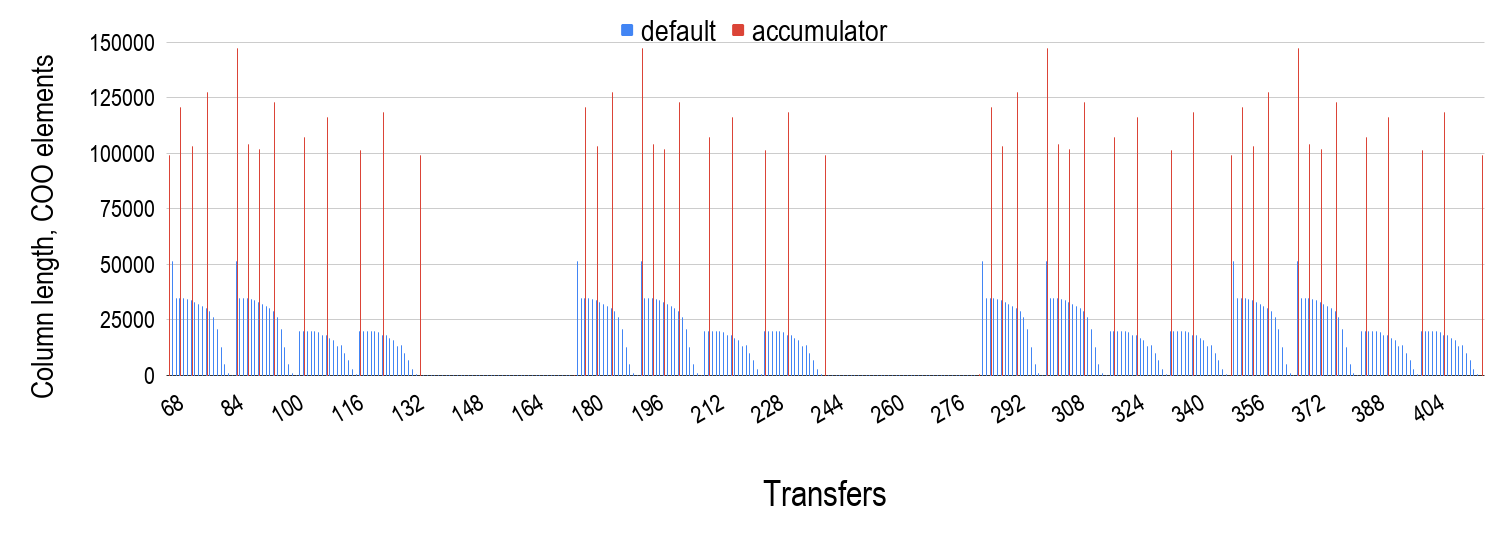
\includegraphics[width=0.9\textwidth]{figures/chapter-3/benchmark-communication-pattern.png}
    \end{figure}
    
    For this particular pattern snippet:
    \begin{itemize}
        \item The amount of data transfers dropped in \textbf{6 times}
        \item From \textbf{344} to \textbf{51}
        \item The average column length increased from \textbf{118114} to \textbf{961186}
        \item or from \textbf{1.8 MB} to \textbf{14.7 MB}
    \end{itemize}

\end{frame}


%%%%%%%%%%%%%%%%%%%%%%%%%%%%%%%%%%%%%%%%%%%%%%%%%%%%%%%%%%
\begin{frame}[t]{Results of Intra-node Allocation}
    \footnotesize
    
    \begin{figure}[htpb]
        \centering
	    \begin{tabular}{c}
		    \subfloat[BM1: blocking MPI; Improved by 9.04\%]{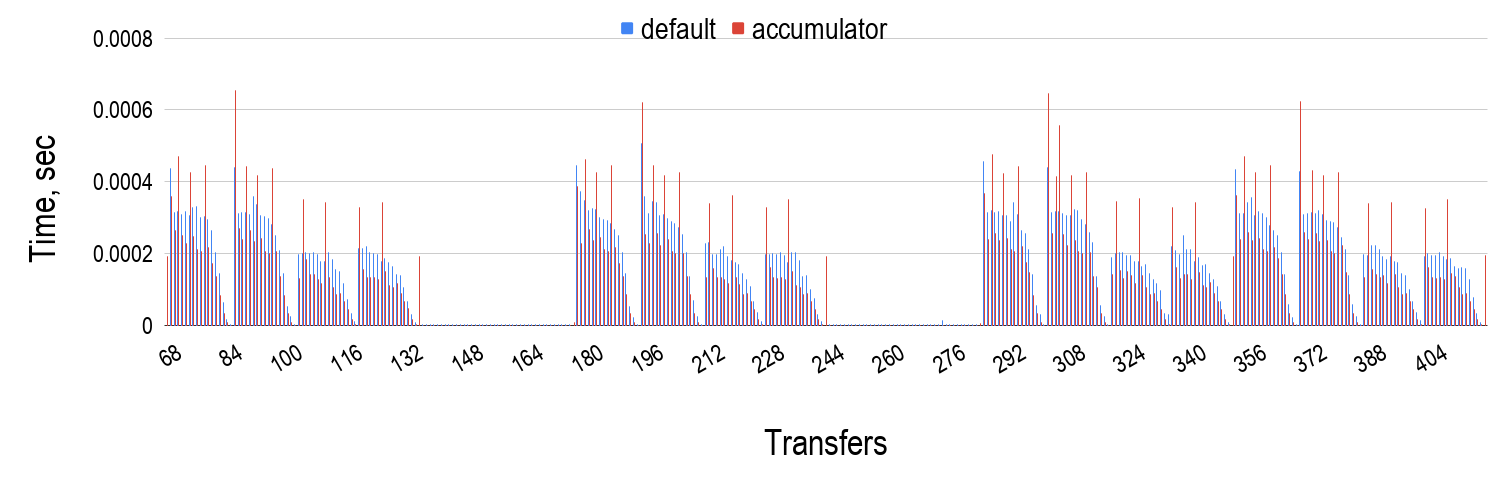
\includegraphics[width=0.7\textwidth]{figures/chapter-3/benchmark-result-blocking.png}} \\
		    \subfloat[BM2: non\-blocking MPI; Improved by  26.26\%]{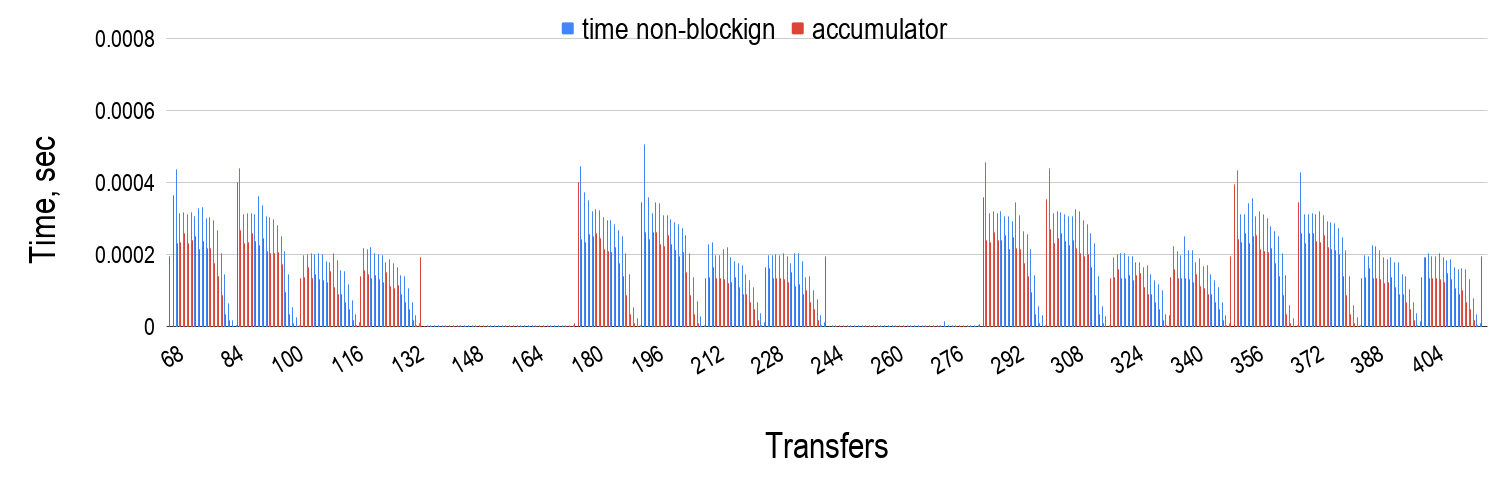
\includegraphics[width=0.7\textwidth]{figures/chapter-3/benchmark-result-non-blocking.png}}
	    \end{tabular}
    	
	\label{fig:benchmark:results-cube-64}
\end{figure}

\end{frame}


%%%%%%%%%%%%%%%%%%%%%%%%%%%%%%%%%%%%%%%%%%%%%%%%%%%%%%%%%%
\begin{frame}[t]{Results of Intra/Inter- Socket/Node Allocation: +}
    \small
    \begin{table}[ht]
    \centering
        \begin{tabular}{|c|c|c|}
        \hline
        \begin{tabular}[c]{@{}c@{}}Benchmark\\ name\end{tabular} & BM1, \% & BM2, \% \\ \hline
    within a socket                                          & 7.61    & 13.84   \\ \hline
    among sockets                                          & 9.04    & 26.26   \\ \hline
    among nodes                                            & -2.06   & 3.20    \\ \hline
    \end{tabular}
    \caption{Time reduction in comparison with the default approach}
        \label{table:benchmark:performance-gain}
    \end{table}
    
    \normalsize
    \begin{itemize}
        \setlength\itemsep{0.5cm}

        \item The new concept \textbf{always} results in some \textbf{performance improvement} 
        \item The \textbf{main} performance \textbf{gain} comes from computation/communication \textbf{overlap}

    \end{itemize}

\end{frame}


%%%%%%%%%%%%%%%%%%%%%%%%%%%%%%%%%%%%%%%%%%%%%%%%%%%%%%%%%%
\begin{frame}[t]{Results of Intra/Inter- Socket/Node Allocation: --}
    \small
    \begin{table}[ht]
    \centering
        \begin{tabular}{|c|c|c|}
        \hline
        \begin{tabular}[c]{@{}c@{}}Benchmark\\ name\end{tabular} & BM1, \% & BM2, \% \\ \hline
    within a socket                                          & 7.61    & 13.84   \\ \hline
    among sockets                                          & 9.04    & 26.26   \\ \hline
    among nodes                                            & -2.06   & 3.20    \\ \hline
    \end{tabular}
    \caption{Time reduction in comparison with the default approach}
    \end{table}
    
    \begin{itemize}
        \item \textbf{Negative effect} of data \textbf{accumulation} in case of \textbf{inter-node} communication
        \item \textbf{Negligible performance gain} out of non-blocking data transfer in case of \textbf{inter-node communication}
        \item \textbf{Specifics} of the benchmark? MPI \textbf{Eager} and \textbf{Rendezvous} protocol switching?
    \end{itemize}

\end{frame}



%%%%%%%%%%%%%%%%%%%%%%%%%%%%%%%%%%%%%%%%%%%%%%%%%%%%%%%%%%
\begin{frame}[t]{Specifics of Benchmarks}
    \small
    \begin{table}[ht]
    \centering
        \begin{tabular}{|c|c|c|}
        \hline
        \begin{tabular}[c]{@{}c@{}}Benchmark\\ name\end{tabular} & BM1, \% & BM2, \% \\ \hline
    within a socket                                          & 7.61    & 13.84   \\ \hline
    among sockets                                          & 9.04    & 26.26   \\ \hline
    among nodes                                            & -2.06   & 3.20    \\ \hline
    \end{tabular}
    \caption{Time reduction in comparison with the default approach}
    \end{table}
    
    \begin{figure}[htpb]
        \centering
        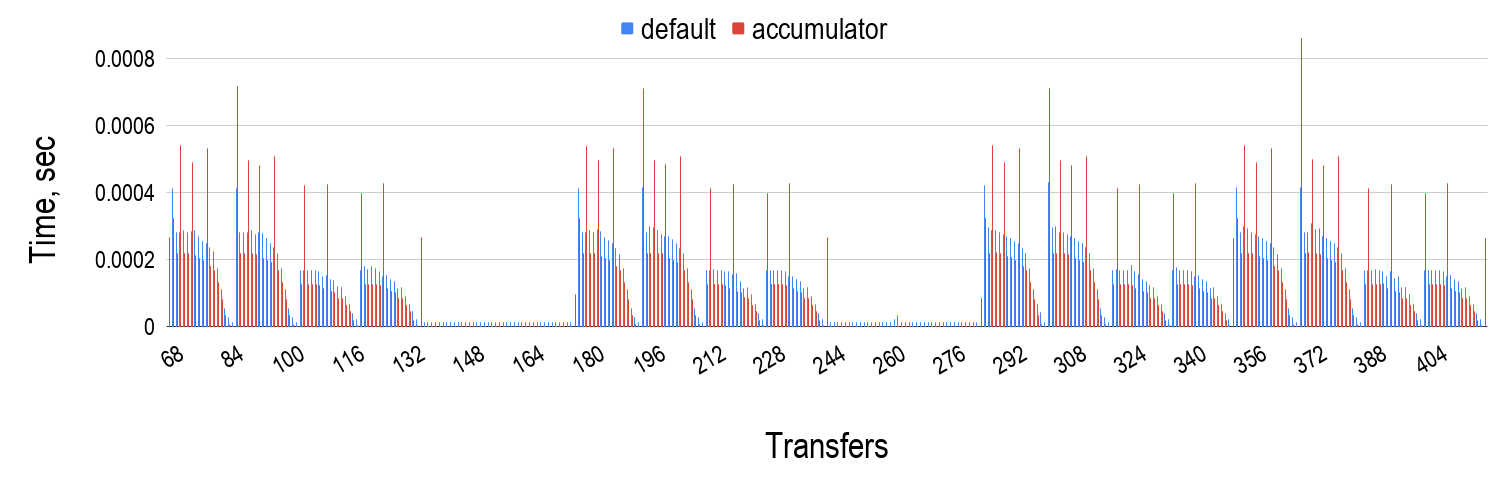
\includegraphics[width=0.8\textwidth]{figures/chapter-3/benchmark-result-non-blocking-inter-node-comm.png}
        \caption{\textbf{Inter-node} communication in case of \textbf{cube-64}}
        \label{fig:benchmark:results-cube-64-inter-node-comm}
\end{figure}
\end{frame}



%%%%%%%%%%%%%%%%%%%%%%%%%%%%%%%%%%%%%%%%%%%%%%%%%%%%%%%%%%
\begin{frame}[t]{Specifics of Benchmarks}
    \small
    \begin{table}[ht]
    \centering
        \begin{tabular}{|c|c|c|}
        \hline
        \begin{tabular}[c]{@{}c@{}}Benchmark\\ name\end{tabular} & BM1, \% & BM2, \% \\ \hline
    within a socket                                          & 7.61    & 13.84   \\ \hline
    among sockets                                          & 9.04    & 26.26   \\ \hline
    among nodes                                            & -2.06   & 3.20    \\ \hline
    \end{tabular}
    \caption{Time reduction in comparison with the default approach}
    \end{table}
    
    \begin{itemize}
        \item Running the benchmarks with \textit{cube-645; N = 100657; F = 1}
        \item size(\textit{cube-645}) $\approx$ 10 $\cdot$  size( \textit{cube-64} )
        \item Performance of BM1 dropped by \textbf{-6.35\%}
        \item Performance of BM2 improved by \textbf{+23.21\%}
    \end{itemize}

\end{frame}

%%%%%%%%%%%%%%%%%%%%%%%%%%%%%%%%%%%%%%%%%%%%%%%%%%%%%%%%%%
\begin{frame}[t]{To consider}
    \justifying
    \small
    \begin{itemize}
        \item Time spent on data transfer is approximately \textbf{one fifth of the total time}
        \item Data transfer happens \textbf{too fast!}
        \item It is just a simple \textbf{benchmark} which \textbf{generates} column vectors filled with \textbf{random numbers}
    \end{itemize}
    
    \begin{figure}[htpb]
        \centering
        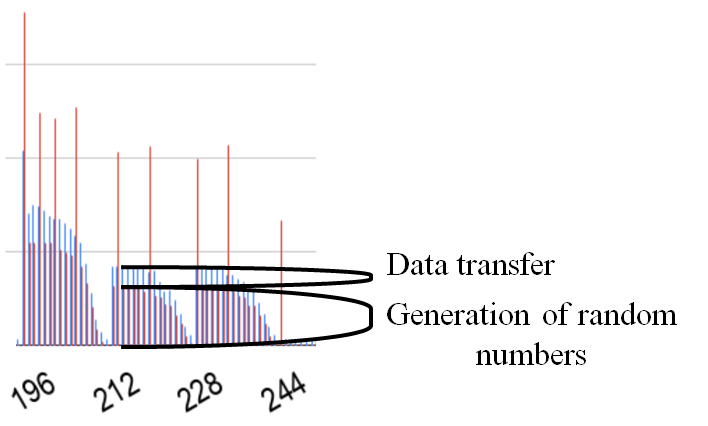
\includegraphics[width=0.6\textwidth]{figures/chapter-3/fast-data-transfer.png}
        \caption{\textbf{Intra-node} communication in case of \textbf{cube-64}}
    \end{figure}

\end{frame}
\fi